\section{APRENDIZAJE PROFUNDO}
    Buscando resolver el problema de la generalización e invarianza a los datos de los que sufren muchos modelos de machine learning o aprendizaje automático, es que nace el Deep Learning o aprendizaje profundo el cual propone apilar múltiples capas con varias neuronas cada una en una red neuronal para lograr representar funciones más complejas y altamente no lineales, a cambio de requerir muchos más datos para su entrenamiento. \citep{Goodfellow-et-al-2016}
    \subsection{PERCEPTRÓN MULTICAPA}
        El perceptrón multicapa, más conocido como red neuronale, extiende la idea de la regresión logística y lineal a un modelo de $n$-etapas, una especie de concatenación de regresiones con la diferencia que a la salida de las capas se les aplica una función $g(\mathbf{X})$ denominada función de activación, que consiste en alguna transformación no lineal de las variables de salida intermedias con el fin de poder realizar ajustes más complejos a los datos. \citep{hastie01statisticallearning}
        
        \begin{figure}[h]
            \centering
%           	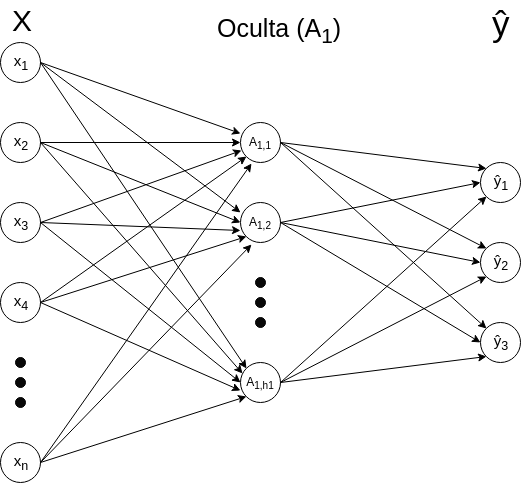
\includegraphics[scale=0.55]{imagenes/NeuralNetwork_bak}
            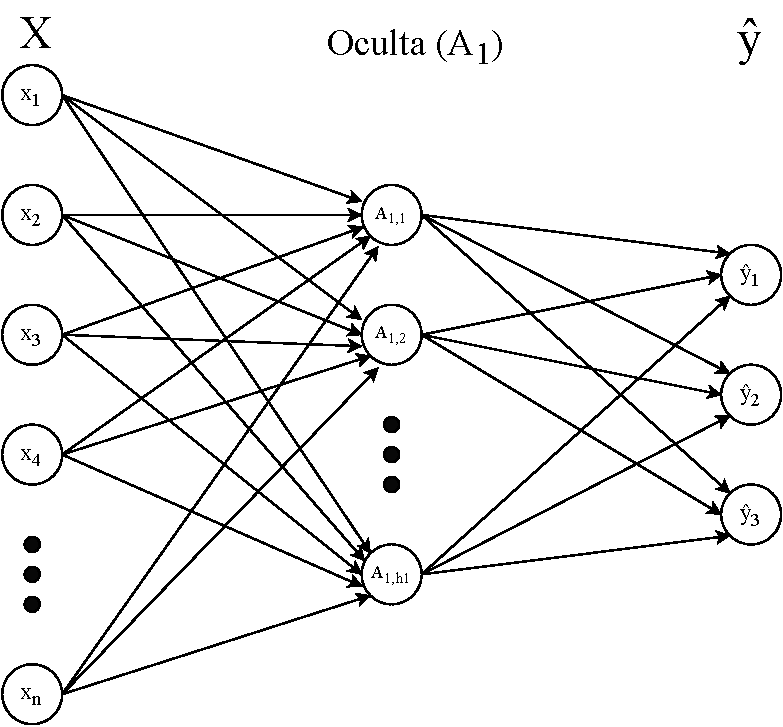
\includegraphics[scale=0.74]{imagenes/NeuralNetwork}
            \caption[Red neuronal con una capa oculta]{Red neuronal con una capa oculta\\Fuente: elaboración propia}
        \end{figure}
        % \vspace{-8mm}
        % \begin{center}
            % Fuente: elaboración propia
        % \end{center}  
        
        Conforme incrementa la cantidad de capas y parámetros de una red neuronal, esta puede aproximar funciones cada vez más complejas, por lo que se le denomina un aproximador universal de funciones, ya que el espacio $\mathcal{H}$ de todas las posibles funciones que puede aproximar, es infinito, es debido a esto que se requieren más observaciones en la muestra de la distribución de datos a modelar. \citep{Goodfellow-et-al-2016}
        
        La red neuronal matemáticamente es una composición de $n$ funciones o capas, aplicando una no linealidad $g(\mathbf{X})$ en cada etapa, con una función de enlace $g(\mathbf{X})$ en la capa de salida, la cual comúnmente es una softmax para clasificación o la identidad para regresión, siendo esta última etapa una regresión logística o lineal respectivamente, con variables de entrada procesadas por las anteriores capas de manera que sea linealmente aproximable en un número arbitrario de dimensiones elegidas por el modelo al entrenarse sobre los datos. La función de costo se denota por $J(\theta)$ con $\theta$ todos los parámetros del modelo. \citep{bishop}
        
        Basándonos en la definición de la matriz $\mathbf{X}$ descrita en el modelo de regresión lineal, la columna de unos agregada antes de ajustar el modelo para el parámetro constante, ahora se considerará como un vector de parámetros $b_k$ para las $l_k$ neuronas de la capa $k$, y los demás parámetros son representados por la matriz $W_k$.
%        Quedando definida la composición de funciones de la red neuronal como:
        
        \begin{equation}
	        \begin{aligned}
	            Z_1 &= X \cdot W_1 + b_1\\
	    		A_1 &= g_1(Z_1) \\
	    		Z_2 &= A_1 \cdot W_2 + b_2 \\
	    		A_2 &= g_2(Z_2) \\
	    		&\dots\\
	    		Z_n &= A_{n-1} \cdot W_n + b_n\\
	    		\hat{Y} &= h(Z_n) \\
	    		J(\theta) &= \sum_{i}^{m} \mathcal{L}(\hat{y_i}, y_i)
	        \end{aligned}
        \end{equation}
        
        
        
        \subsubsection{FUNCIONES DE ACTIVACIÓN}
        Con el fin de obtener aproximaciones no lineales a los datos, se debe evaluar la salida $Z_k$ de cada capa en una función de activación no lineal $g_k(Z_k)$.
        
        Las funciones de activación más comúnmente usada por ser fácil de computar y diferenciar es la \textit{Rectified Linear Unit} o \textbf{RELU} \citep{Goodfellow-et-al-2016}, la cual está definida por:
        \begin{equation}
            g(Z_k) = max(0, Z_k) \text{ $\forall$ $z_{k,j}$ / $j$ : $0, 1, ..., l_k$}
        \end{equation}
        
        \noindent cuya derivada con fines de estabilidad numérica es
        
        \begin{equation}
			\frac{\partial g(Z_k)}{\partial Z_k} = 
			\begin{cases}
			\text{1 si } z_{k,j} > 0\\
			\text{0 en otro caso}
			\end{cases}
		\end{equation}
        
        \subsubsection{RETROPROPAGACIÓN DE LOS ERRORES}
        Para ajustar los parámetros o entrenar la red neuronal, al tener más capas por las que pasar para obtener todos los gradientes de los errores, se debe derivar a través de cada una de ellas, a este algoritmo se le llama Backpropagation o Retropropagación, que es simplemente como su nombre dice, propagar los gradientes de reverso a través de la red neuronal.
		
		Primero se obtiene la derivada con respecto da cada uno de los parámetros de la composición de funciones por regla de la cadena
		
		\begin{equation}
		    \frac{\partial J}{\partial \theta_k} = \frac{\partial J}{\partial Z_n} \cdot  \frac{\partial Z_{n}}{\partial A_{n-1}} \cdot \frac{\partial A_{n-1}}{\partial Z_{n-1}} \cdot  \dots \cdot \frac{\partial A_{k}}{\partial Z_{k}} \cdot \frac{\partial Z_{k}}{\partial \theta_{k}}
		\end{equation}
		
		\noindent dónde $\theta_k$ representa cualquiera de los parámetros de $W_k$ o $b_k$ en la capa $k$, notese que para obtener la derivada con respecto de los parámetros en la capa $k$ se requiere la derivada en con respecto de las activaciones las capas siguientes, así, cuando se obtiene la derivada con respecto de los parámetros de la capa $k$ ya se calcula para todas las capas siguientes y sólo se debe multiplicar por la derivada de la salida lineal de la capa $k$ con respecto del parámetro $\theta_k$. \citep{bishop}
		
		Para el caso de regresión y clasificación con softmax $\frac{\partial J}{\partial Z_n} = (\mathbf{\hat{Y}} - \mathbf{Y})$ de forma vectorial, de manera general la derivada con respecto de algún parámetro está dada por
		
		\begin{equation}
		    \frac{\partial J}{\partial \theta_k} = \frac{\partial J}{\partial Z_n} \cdot \prod_{i=0}^{n-(k+1)} W_{n-i} \frac{\partial g_{n-(i+1)}(Z_{n-(i+1)})}{\partial Z_{n-(i+1)}} \cdot \frac{\partial Z_k}{\partial \theta_k}
		\end{equation}
		
		Similar a la regresión logística, se estiman los parámetros mediante un método de optimización, cuyo requisito sea la derivada con respecto a cada uno de los parámetros.
		
    \subsection{REDES NEURONALES CONVOLUCIONALES}
        Es un tipo de arquitectura de redes neuronales diseñada específicamente para tareas sobre imágenes, de manera que las operaciones sobre las observaciones de entrada ya no son composiciones realizando multiplicaciones matriciales, sino que cada neurona se convierte en un filtro o kernel de dimensiones $(k \times k)$, de los cuales se tienen varios filtros que se aplican sobre la imagen mediante la convolución.
        
        La idea detrás de este tipo de red es que se apliquen varios filtros en cada capa de la red para extraer características importantes de los objetos que se buscan, estos filtros se aprenden mediante retropropagación y ya no se diseñan a mano \citep{Goodfellow-et-al-2016}.
        
        \begin{figure}[H]
            \centering
            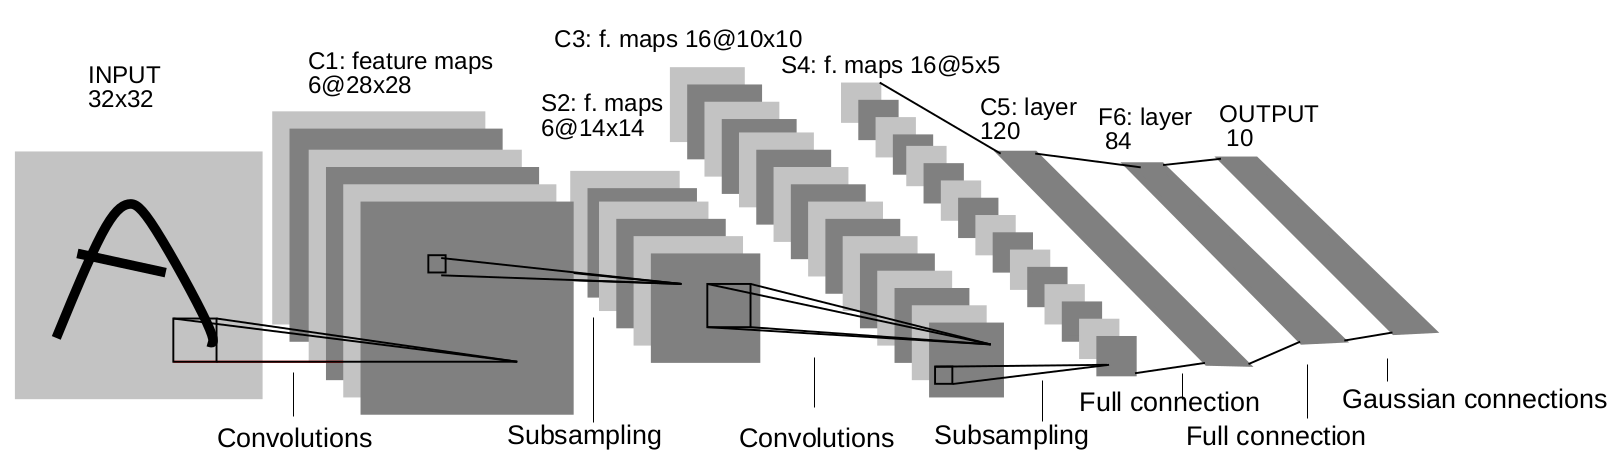
\includegraphics[scale=0.25]{imagenes/lenet}
            \caption[Red neuronal convolucional para la clasificación de dígitos manuscritos]{Red neuronal convolucional para la clasificación de dígitos manuscritos\\ Fuente: \citep{lecun-gradientbased-learning-applied-1998}}
        \end{figure}
        % \vspace{-8mm}
        % \begin{center}
        %     Fuente: \citep{lecun-gradientbased-learning-applied-1998}
        % \end{center}
        
        \subsubsection{STRIDES}
        Cuando se desea optimizar la operación sacrificando representabilidad o disminuir la muestra, se puede incrementar el tamaño del salto de la ventana deslizante al convolucionar la imágen con el filtro, a este salto se le llama \textbf{stride}
        
        
        Aplicando esta idea, se obtiene una fórmula general para calcular la dimensión de la matriz resultante al aplicar cada uno de los filtros con un stride $s$
        
        $$\frac{I_{alto} - k + s}{s} \times \frac{I_{ancho} - k + s}{s}$$ 
        
        \begin{figure}[H]
            \centering
            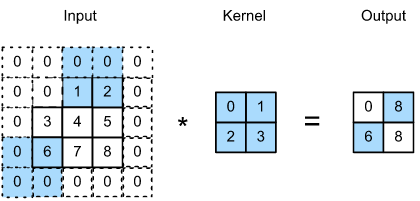
\includegraphics[scale=0.55]{imagenes/stride}
            \caption[Convolución con $s=2$]{Convolución con $s=2$\\ Fuente: \citep{zhang2020dive}}
        \end{figure}
        % \vspace{-8mm}
        % \begin{center}
        %     Fuente: \citep{zhang2020dive}
        % \end{center}
        \subsubsection{POOLING}
        Es una operación sobre la entrada bidimensional que con un stride $s$ recorre una ventana deslizante de dimensión $p \times p$ extrayendo información característica de cada sección de la entrada.
        
        Existen dos tipos de pooling más comunes, average pooling que promedia los valores activados en cada sección de la imágen sobre la que pasa la ventana y max pooling, el cual extrae el elemento más representativo, es decir el con mayor valor, de cada sección de la imágen.
        
        \begin{figure}[H]
            \centering
            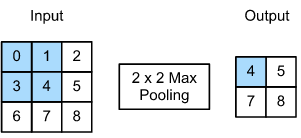
\includegraphics[scale=0.6]{imagenes/pooling}
            \caption[Pooling con con $s=1$]{pooling con con $s=1$\\ Fuente: \citep{zhang2020dive}}
        \end{figure}
        
        \subsubsection{MOBILENET V2}
        	Muchas tareas de aprendizaje profundo se despliegan en dispositivos con poco poder de cómputo, las redes neuronales con mejores resultados tienden a tener cada vez más capas y ser más costosas de computar, es por eso que nacen alternativas como la MobileNet, pensada para ejecutarse en dispositivos móviles y embedidos, sacrificando exactitud de predicción por velocidad, aún así obteniendo buenos resultados.
        	
        	La idea principal, es separar las convoluciones en dos etapas, la primera etapa llamada DepthWise Convolution, consiste en convolucionar la entrada de dimensiones $h\times w\times c$ con $c$ filtros de dimensiones $k\times k$, para obtener una salida de dimensiones $\frac{h}{s}\times\frac{w}{s}\times c$, con $s$ los strides de la convolución. La segunda etapa llamada PointWise Convolution recibe la salida de la DepthWise Convolution y le aplica $d$ filtros de dimensiones $1\times 1\times c$, para apilar las salidas y obtener finalmente una salida $\frac{h}{s}\times\frac{w}{s}\times d$.
        	
        	Este mismo resultado se puede obtener mediante una convolución con profundidad por definición, aplicando $d$ filtros de dimensión $k\times k\times c$, sin embargo el número de operaciones es mayor, ya que se realizan $\frac{h}{s}\cdot \frac{w}{s}\cdot c\cdot k^2\cdot d$ operaciones, comparadas con las $\frac{h}{s}\cdot \frac{w}{s}\cdot k^2\cdot c + \frac{h}{s}\cdot \frac{w}{s}\cdot 1^2\cdot c\cdot d = \frac{h}{s}\cdot \frac{w}{s}\cdot c\cdot(k^2 + d)$ operaciones de las convoluciones separables de la MobileNet.
        	
        	\begin{figure}[H]
        		\centering
        		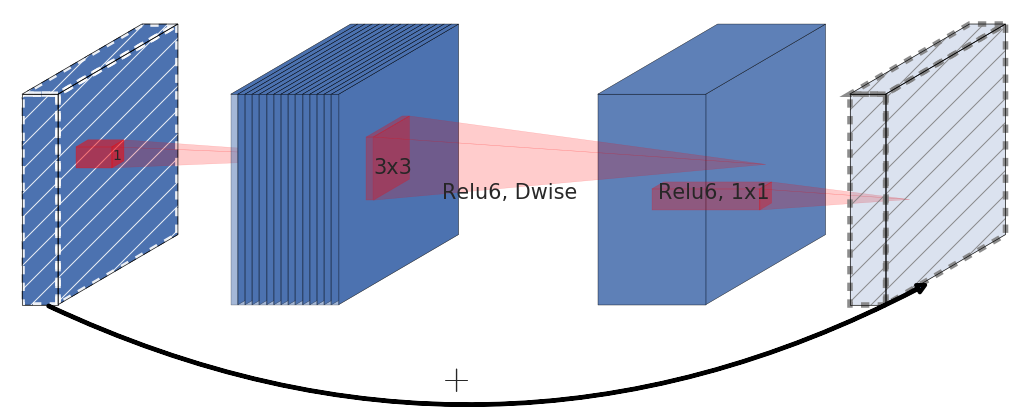
\includegraphics[scale=0.25]{imagenes/bottleneck}
        		\caption[Cuello de botella residual]{cuello de botella residual (residual bottleneck) Fuente:\citep{8578572}}
        		\label{bottleneck}
        	\end{figure}
        	
        	En base esta nueva convolución, se proponen bloques denominados cuellos de botella residuales detallados en la figura \ref{bottleneck}, que consisten en una capa PointWise con no linealidad Relu truncada con valor máximo 6 llamada Relu6 para obtener $t\cdot k$ filtros (con $t$ llamado el factor de expansión y $k$ la dimensión del filtro $k\cdot k$), seguido de una capa DepthWise $3\times3$ con stride $s$ y Relu6, para pasar por otra capa PointWise sin activación no lineal y que devuelve $d$ filtros. El término residual se refiere a que existe una conexión extra que envío directamente la salida de la primera PointWise Convolution a la última para sumarse de manera ponderada, con el fin de prevenir el desvanecimiento de los gradientes durante el entrenamiento \citep{8578572}.
        	
        
        	Usando estos bloques, se construye la arquitectura MobilenetV2 descrita en la tabla \ref{mobilenet2}
        	
        	\begin{center}
        		\footnotesize
        		\begin{tabular}{|c|c|c|c|c|c|}
        			\hline
					Entrada & Operador & Factor $t$ & Canales $c$ & Repeticiones $n$ & Stride $s$\\
					\hline
					$224^2\times3$ & conv2d & - & 32 & 1 & 2\\
					$112^2\times32$ & bottleneck & 1 & 16 & 1 & 1\\
					$112^2\times16$ & bottleneck & 6 & 24 & 2 & 2\\
					$56^2\times24$ & bottleneck & 6 & 32 & 3 & 2\\
					$28^2\times32$ & bottleneck & 6 & 64 & 4 & 2\\
					$14^2\times64$ & bottleneck & 6 & 96 & 3 & 1\\
					$14^2\times96$ & bottleneck & 6 & 160 & 3 & 2\\
					$7^2\times160$ & bottleneck & 6 & 320 & 1 & 1\\
					$7^2\times320$ & conv2d $1\times1$ & - & 1280 & 1 & 1\\
					$7^2\times1280$ & average pooling $7\times7$ & - & - & 1 & -\\
					$1^2\times1280$ & conv2d $1\times1$ & - & \#clases & - & -\\
        			\hline
        		\end{tabular}
        		\captionof{table}[MobileNet V2]{MobileNet V2 Fuente:\citep{8578572}}\label{mobilenet2}
        	\end{center}
        \subsubsection{FAST DEPTH}
        	Una de las áreas abiertas de investigación mediante redes neuronales convolucionales es la de inferencia de profundidad dada una imagen. A diferencia de los métodos de visión estéreo que mediante dos cámaras permite estimar la distancia de objetos al observador, esta tarea pretende hacerlo con una sola cámara, para esto se requiere de una arquitectura Encoder-Decoder, es decir una red codificadora que reciba la imagen RGB como entrada y extraiga las características más importantes de esta en un vector, luego otra red decodificadora, recibe como entrada este vector y devuelve la como salida una nueva imagen dependiendo de la tarea a resolver.
        	
        	Normalmente para este tipo de problemas se usan redes complejas con alto poder de abstracción, sin embargo para tareas con limitado poder de cómputo se debe simplificar la arquitectura, es así que nace la idea de la red FastDepth una red convolucional de código libre disponible en el repositorio de github de los autores \citep{icra_2019_fastdepth}.
        	
        	Esta red propone usar una mobilenet v1 como encoder y una nueva red decoder de 5 capas, este decodificador aplica una convolución DepthWise con bordes de relleno para obtener el mismo tamaño de salida, y PointWise para los filtros nuevos, luego de cada convolución se realiza una interpolación por vecinos más cercanos para duplicar el tamaño, hasta llegar a la última capa dónde se aplica solamente una convolicion PointWise.
        	
        	\begin{figure}[H]
        		\centering
        		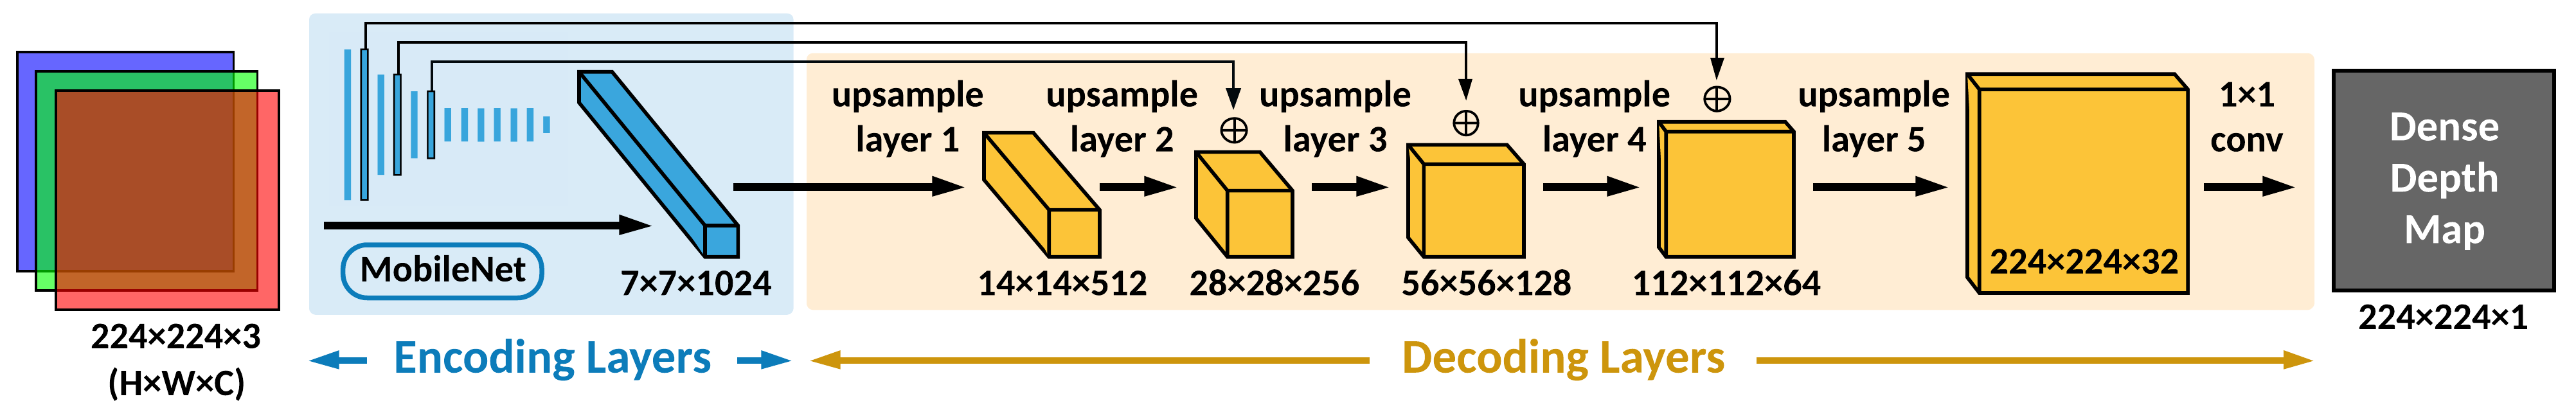
\includegraphics[scale=0.11]{imagenes/fastdepth}
        		\caption[Arquitectura FastDepth]{arquitectura FastDepth\\ Fuente: \citep{icra_2019_fastdepth}}\label{fastdepth}
        	\end{figure}
        	
        	La salida de esta red es una matriz de $224\times224$ con las estimaciones de distancia para cada píxel RGB de entrada.
        	
        	Como especifica la figura \ref{fastdepth} se tienen también conexiones residuales, o skip connections, que similar a los bloques de la mobilenet v2, permiten realizar saltos entre las conexiones de las capas mediante una suma ponderada a la capa resultante para así prevenir gradientes ceros durante el entrenamiento, debido a la forma de U de estas conexiones, a esta arquitectura se la denomina U-Net.
    \subsection{APRENDIZAJE DE REPRESENTACIONES PROFUNDAS}
	    En cada etapa de la red neuronal se extraen características representativas de la imagen que ayuden a realizar la predicción de la tarea para la cual se la entrena, conforme pasan más etapas en la red los filtros buscan características más específicas \citep{Goodfellow-et-al-2016}
	    
	    \begin{figure}[H]
 	        \centering
 	        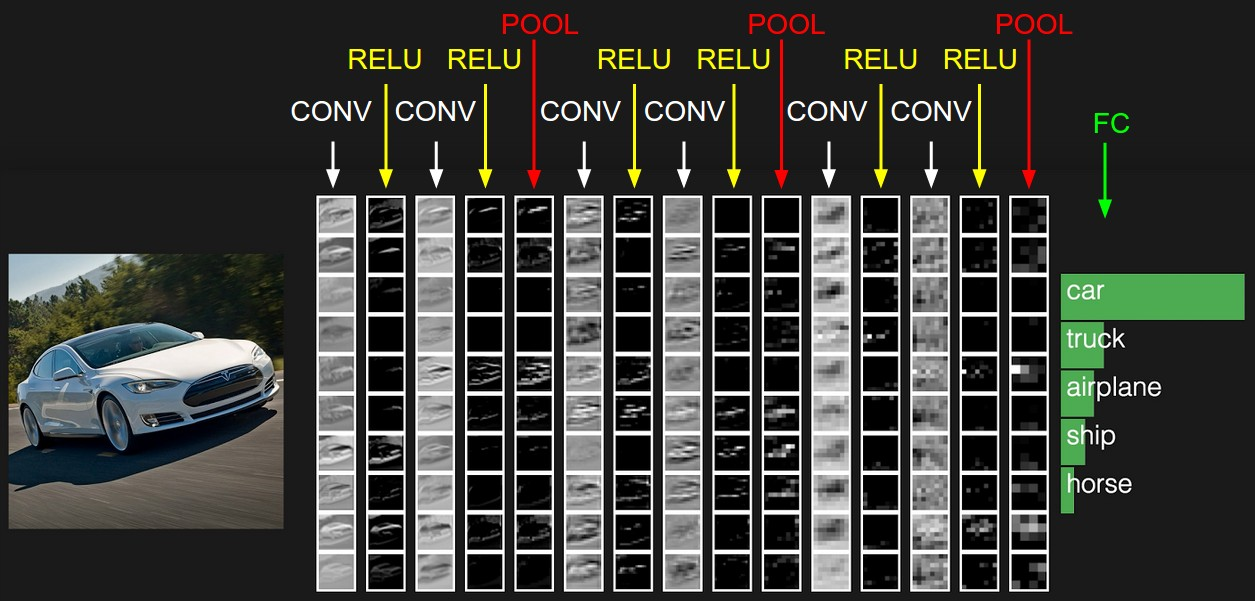
\includegraphics[scale=0.23]{imagenes/convnet}
 		    \caption[Extracción de las características profundas aprendidas]{Extracción de las características profundas aprendidas\\ Fuente: \citep{stanford_2020}}
	    \end{figure}

	    
	    \noindent de esta manera activando (dando valores altos) a ciertas partes de la imagen que es donde ``presta atención'' en busca de los objetos que desee clasificar o en base a los que predecir algún valor numérico, a esto se le llama aprendizaje de representaciones profundas, porque los filtros aprenden información desde bajo a alto nivel que caracterice los objetos en las etiquetas de entrenamiento.
		
		\begin{figure}[H]
			\centering
			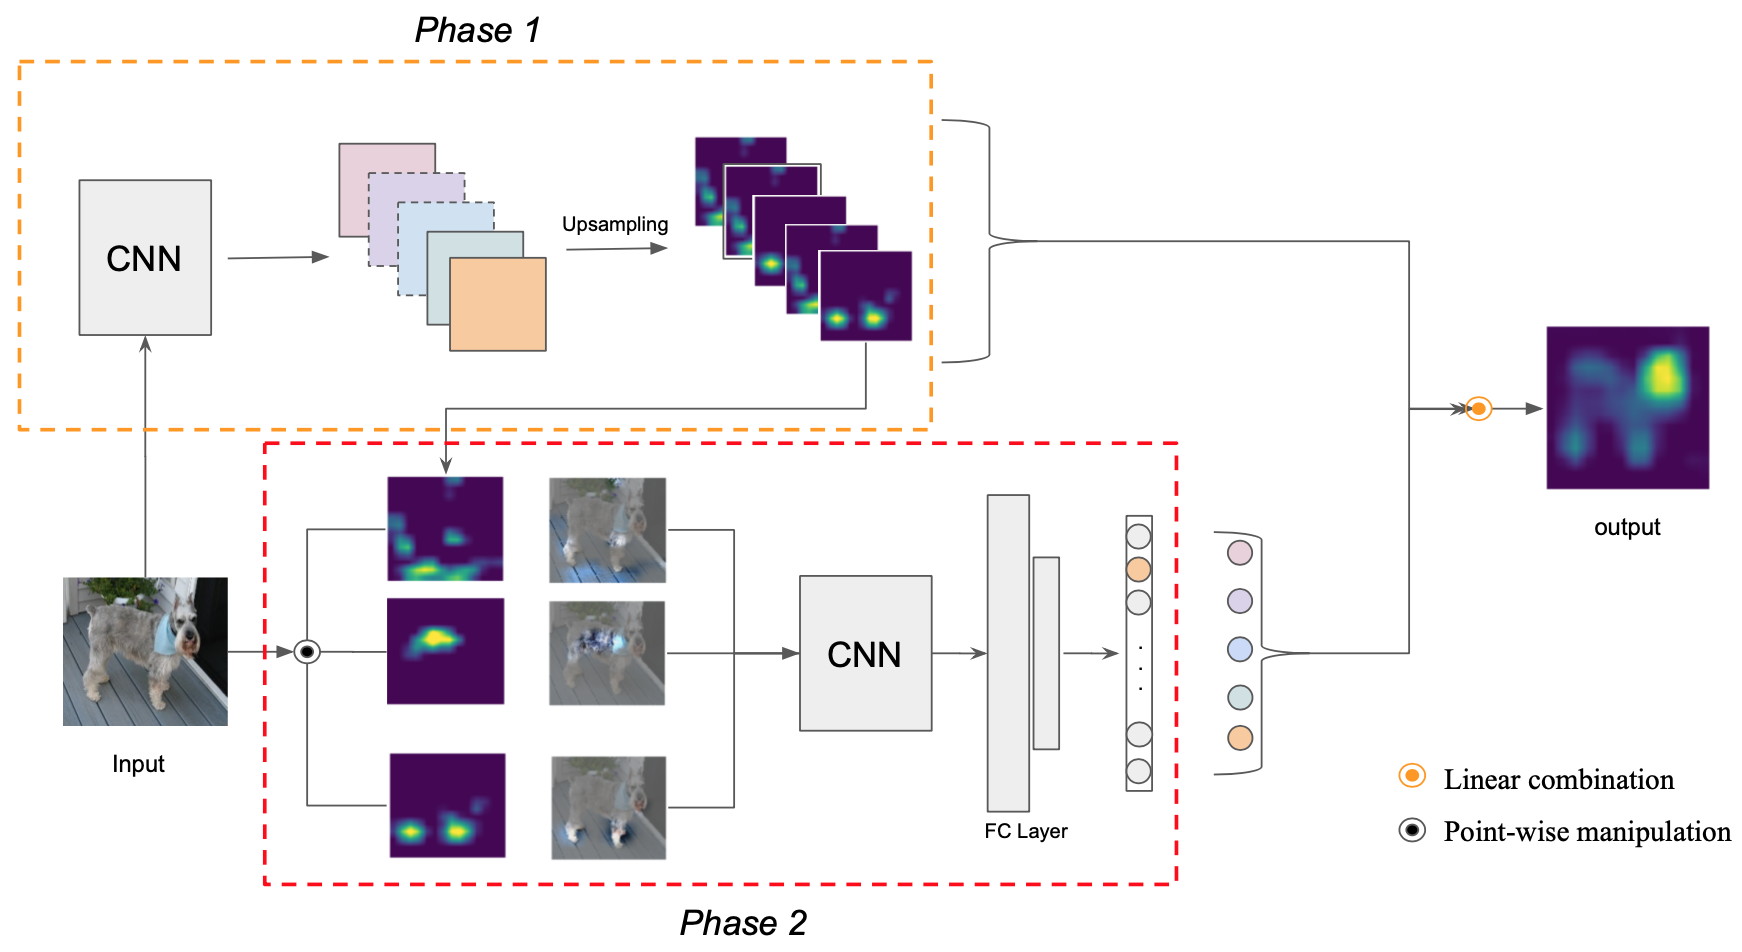
\includegraphics[scale=0.25]{imagenes/scorecam_net}
			\caption[Algoritmo ScoreCam]{algoritmo ScoreCam\\Fuente:\citep{Wang_2020_CVPR_Workshops}}\label{scorecam}
		\end{figure} 
		
		Uno de los algoritmos utilizados para esta tarea es ScoreCam, el cual calcula un mapa de prominencia dadas las capas activadas al evaluar una imagen por toda la red descrita en la figura \ref{scorecam}. Para lograrlo primero pasa la imagen por la red e intercepta la salida de la última capa convolucional, iterando por sus filtros. En cada iteración para el filtro i-ésimo, realiza un cambio de tamaño mediante interpolación para que el filtro tenga las mismas dimensiones de la imagen original, luego normaliza sus valores activados y los multiplica por la imagen original para re ingresar a la red, se captura la salida de la clase deseada y se acumula ponderando por la clase los valores del filtro por iteración, para finalmente realizar un cambio de tamaño a la variable acumulada y combinar con la imagen original para poder visualizar las áreas de interés de la imagen para la red.